\documentclass[a4paper]{article}

\usepackage{fullpage}

\usepackage{graphicx}
\usepackage{subcaption}

\usepackage{amsmath}
\usepackage{tabularx}

% Code for typesttting C code
\usepackage{listings}
\usepackage{color}

\definecolor{mygreen}{rgb}{0,0.6,0}
\definecolor{mygray}{rgb}{0.5,0.5,0.5}
\definecolor{mymauve}{rgb}{0.58,0,0.82}
\definecolor{mybrown}{rgb}{0.5,0,0}

\lstdefinestyle{MyCStyle}{ %
  language=C,                      % the language of the code
  backgroundcolor=\color{white},   % choose the background color; you must add \usepackage{color} or \usepackage{xcolor}
  basicstyle=\ttfamily    ,        % the size of the fonts that are used for the code
  breakatwhitespace=false,         % sets if automatic breaks should only happen at whitespace
  breaklines=true,                 % sets automatic line breaking
  captionpos=b,                    % sets the caption-position to bottom
  commentstyle=\color{mygreen},    % comment style
  deletekeywords={...},            % if you want to delete keywords from the given language
  escapeinside={\%*}{*)},          % if you want to add LaTeX within your code
  extendedchars=true,              % lets you use non-ASCII characters; for 8-bits encodings only, does not work with UTF-8
  frame=single,                    % adds a frame around the code
  keepspaces=true,                 % keeps spaces in text, useful for keeping indentation of code (possibly needs columns=flexible)
  keywordstyle=\color{blue},       % keyword style
  morecomment=[l][\color{mybrown}]\#,  % compiler directive
  morekeywords={*,...},            % if you want to add more keywords to the set
  numbers=left,                    % where to put the line-numbers; possible values are (none, left, right)
  numbersep=5pt,                   % how far the line-numbers are from the code
  numberstyle=\tiny\color{mygray}, % the style that is used for the line-numbers
  rulecolor=\color{black},         % if not set, the frame-color may be changed on line-breaks within not-black text (e.g. comments (green here))
  showspaces=false,                % show spaces everywhere adding particular underscores; it overrides 'showstringspaces'
  showstringspaces=false,          % underline spaces within strings only
  showtabs=false,                  % show tabs within strings adding particular underscores
  stepnumber=1,                    % the step between two line-numbers. If it's 1, each line will be numbered
  stringstyle=\color{mymauve},     % string literal style
  tabsize=2,                       % sets default tabsize to 2 spaces
  title=\lstname                   % show the filename of files included with \lstinputlisting; also try caption instead of title
}

\newlength{\pic}

\begin{document}

\title{EE445M Lab 6 Report}
\author{\bfseries Yen-Kai Huang, Siavash Zanganeh Kamali, Chen Cui, Miao Qi, Yan Zhang}
\maketitle

\section{Objective} The goal of this lab is to prepare for the final Robot race. In this lab we will interface various
components, including Ping)))) ultrasonic distance sensor, IR distance sensor, and DC motor. A layered communication system
using CAN protocol will transmit the information between two microcontrollers. We will design and implement a software
communication protocol to transmit the sensor data and other things.

In this lab we will also form a team of 4 or 5, which requires us also to apply communication skills to function as a team.

\section{Hardware Design}
%\noindent Ping ultrasonic sensor is shown at Figure-\ref{ping}
\setlength{\pic}{0.8\textwidth}
\begin{figure}[htp]
\noindent Ping sensor is shown at Figure-\ref{ping}
\center
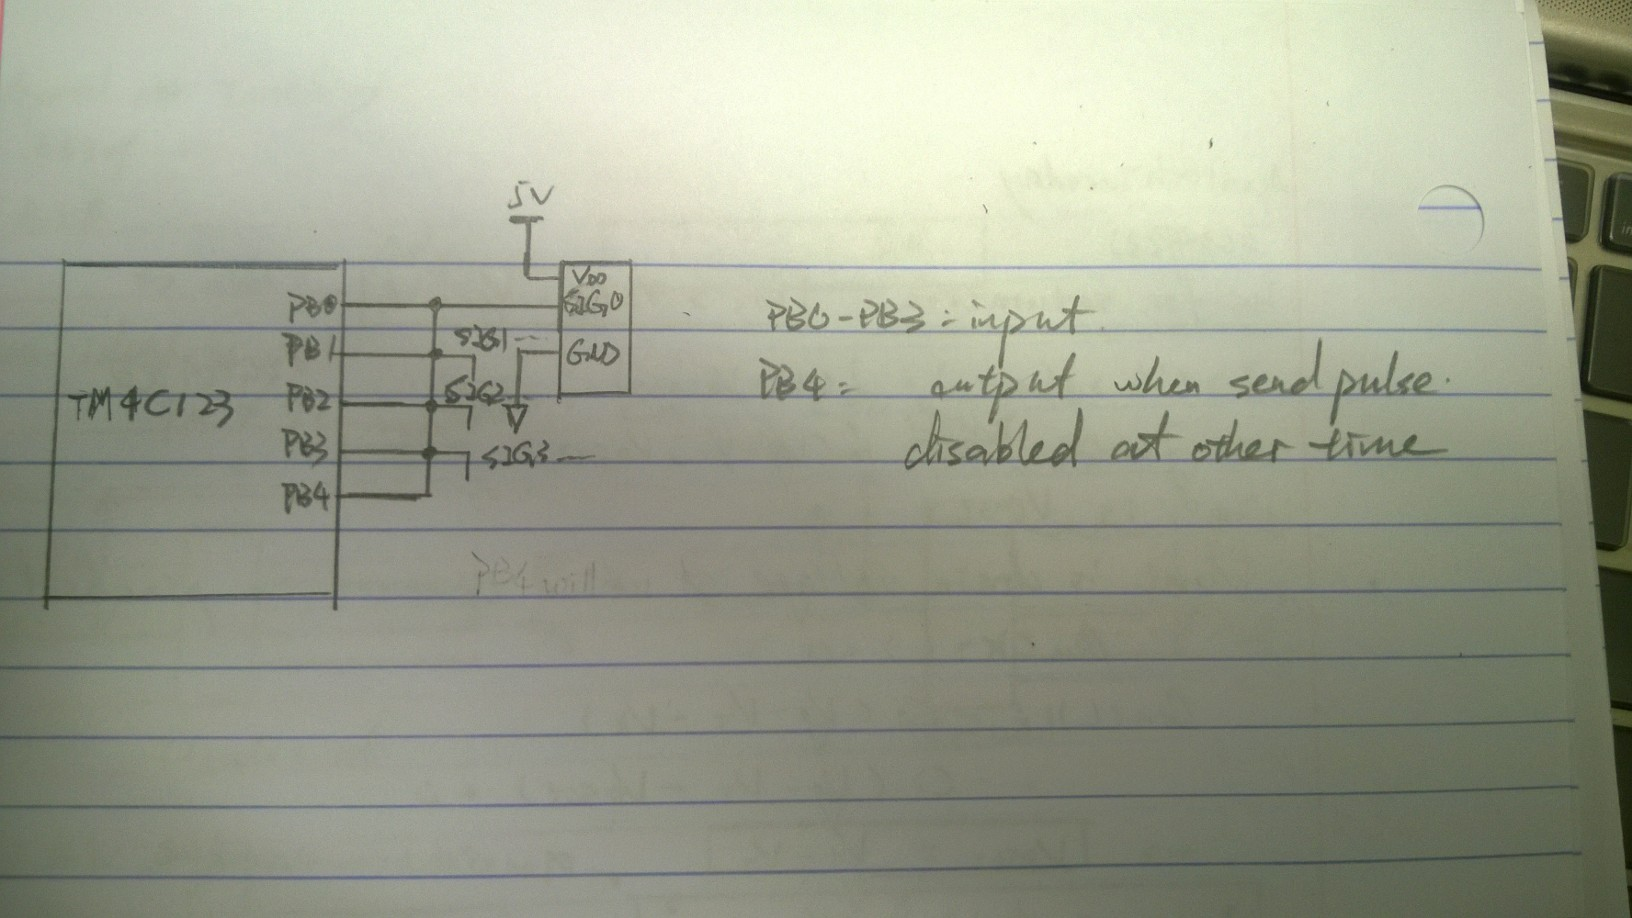
\includegraphics[width=\pic]{circuits/Ping_Circuit}
\caption{ }
\label{ping}
\end{figure}

IR sensor is shown at Figure-\ref{ir}

\setlength{\pic}{0.8\textwidth}
\begin{figure}[htp]
\center
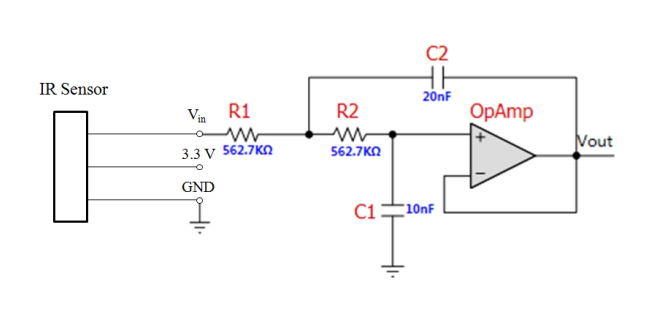
\includegraphics[width=\pic]{circuits/IR_Circuit}
\caption{ }
\label{ir}
\end{figure}

The DC motor circuit is shown at Figure-\ref{motor}

\setlength{\pic}{0.8\textwidth}
\begin{figure}[htp]

\center
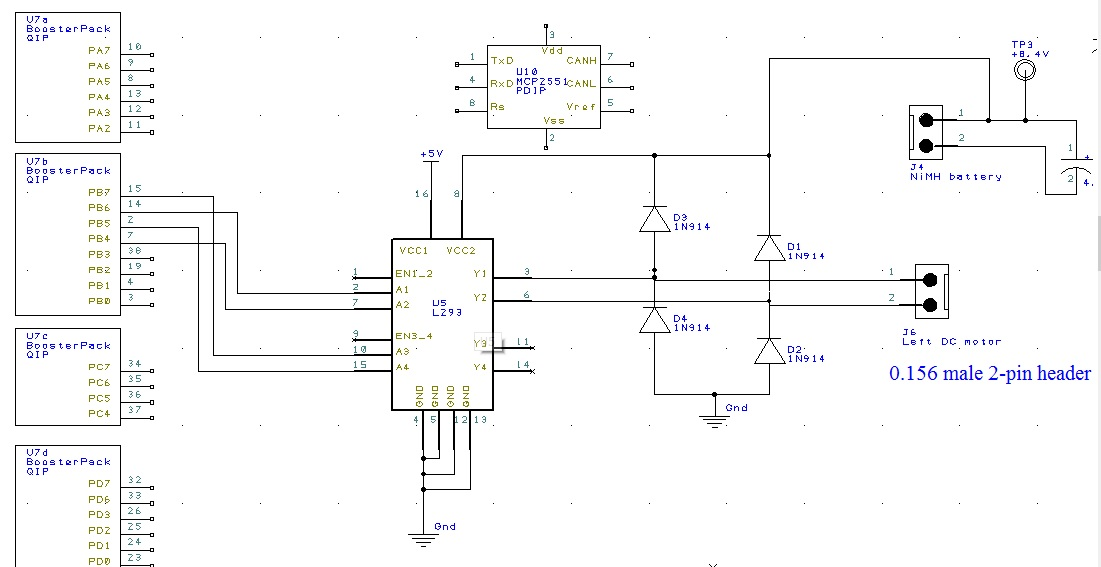
\includegraphics[width=\pic]{circuits/PWM_Circuit}
\caption{ }
\label{motor}
\end{figure}

\newpage

\section{Software Design} 

\paragraph{(a)} We made small changes to \texttt{CAN0.c}, replacing the spinlock  mechanism with actual semaphore.

\lstset{language=C, style=MyCStyle}
\lstinputlisting{code/can0.c}

We also modified the FIFO macro to internally include semaphores.

\lstinputlisting{code/FIFO_sema4.h}

\paragraph{(b)} IR sensor code is basically the same as Lab.\ 4, except that I decoupled the \texttt{Filter()} functions
from the filter buffer. The call-back functions in ADC routine is now responsible for acquiring and storing the data.

\lstinputlisting{code/ir_sensor.h}
\lstinputlisting{code/ir_sensor.c}

For the Ping))) interfacing, we used one pin to output the $ 5 \, \mu s$ pulse, and one pin for each sensor set to
trigger an interrupt at both edges. The handler will calculate the difference of time between the two edges and thus
determine the distance measurement.

\lstinputlisting{code/ping.h}
\lstinputlisting{code/ping.c}

\paragraph{(c)} The code that sets up the distributed data acquisition system comes in two sides. On the transmitter side,
the \texttt{main} initializes the sensors and network, and sends data periodically at about $ 10 \, Hz $.

\lstinputlisting{code/main_TX.c}

On the receiver side, the \texttt{main} initializes the display and network, then add a thread that waits for the packet
from the network. Once it receives a packet, it checks the packet ID to determine the type of data and then publish it
to the display.

\lstinputlisting{code/main_RX.c}

This is a very simplistic example, however, it contains the full range of function for a distributed Data Acquisition System.

\section{Measurement}

\paragraph{(a) Ping))) Calibration}	Ping measurements in Table-\ref{tab1}
\begin{table}
\tiny
\center
  \begin{tabular}{|c|c|c|c|c|c|c|c|c|c|c|}
    \hline
    \multicolumn{11}{|c|}{Ping measurements} \\
    \hline
   Truth dT(cm) & \multicolumn{8}{|c|}{measured dM(cm)} & standard deviation & span \\
    \hline
    10 & 10.1538 & 10.2742 & 10.129 & 10.2398 & 9.9102 & 10.1231 & 10.2314 & 9.9324 & 0.136715993 & 0.364\\
	20 & 20.7653 & 20.9498 & 20.4286 & 20.5348 & 20.8695 & 21.0135 & 20.8493 & 20.9756 & 0.212323325 & 0.5849\\
	30 & 31.4354 & 31.2317 & 31.2342 & 31.5463 & 31.8467 & 31.6756 & 31.3765 & 31.0475 & 0.260240679 & 0.7992\\
	50 & 52.7532 & 52.8654 & 52.2543 & 52.7397 & 52.9485 & 53.0123 & 52.9475 & 53.2397 & 0.286319955 & 0.9854\\
	80 & 83.1323 & 82.1398 & 83.2538 & 84.0132 & 83.8764 & 83.1233 & 82.4956 & 83.2835 & 0.626714781 & 1.8734\\
    \hline
  \end{tabular}
  \caption{Ping measurements}
  \label{tab1}
\end{table}

%\begin{table}[htbp]
%  \tiny
%  \centering
%  \caption{Ping measurements \textbf{cm}}
%  \begin{tabularx}{\textwidth}{|X|X|X|X|X|X|X|X|X|X|X|}
%  \hline
%  \multicolumn{11}{|c|}{Ping measurements} \\
%  Truth dT(cm0) & \multicolumn{8}{|c|}{measured dM(cm)} & standard deviation & span \\
%  \hline
%    10 & 10.1538 & 10.2742 & 10.129 & 10.2398 & 9.9102 & 10.1231 & 10.2314 & 9.9324 & 0.136715993 & 0.364\\
%	20 & 20.7653 & 20.9498 & 20.4286 & 20.5348 & 20.8695 & 21.0135 & 20.8493 & 20.9756 & 0.212323325 & 0.5849\\
%	30 & 31.4354 & 31.2317 & 31.2342 & 31.5463 & 31.8467 & 31.6756 & 31.3765 & 31.0475 & 0.260240679 & 0.7992\\
%	50 & 52.7532 & 52.8654 & 52.2543 & 52.7397 & 52.9485 & 53.0123 & 52.9475 & 53.2397 & 0.286319955 & 0.9854\\
%	80 & 83.1323 & 82.1398 & 83.2538 & 84.0132 & 83.8764 & 83.1233 & 82.4956 & 83.2835 & 0.626714781 & 1.8734\\
%    \hline
%    \end{tabularx}%
%  \label{tab:addlabel}%
%\end{table}%


\paragraph{(b) IR sensor Calibration}	IR sensor measurements in Table-\ref{tab2}

\begin{table}
\tiny
\center
  \begin{tabular}{|c|c|c|c|c|c|c|}
    \hline
    \multicolumn{7}{|c|}{IR sensor measurements} \\
    \hline
    Truth dT(c0) & ADC average & ADC Std. Dev. & ADC span & Voltage average(V) & Voltage Std. Dev.(V) & Voltage span (V)\\
    \hline
	10 & 2822 & 5 & 19 & 2.067 & 0.004 & 0.014\\
	15 & 1979 & 4 & 15 & 1.450 & 0.003 & 0.011\\
	20 & 1570 & 5 & 19 & 1.150 & 0.003 & 0.014\\
	25 & 1282 & 6 & 25 & 0.939 & 0.005 & 0.018\\
	30 & 1114 & 5 & 27 & 0.816 & 0.004 & 0.020\\
	35 & 941 & 2 & 8 & 0.689 & 0.001 & 0.006\\
	40 & 848 & 7 & 23 & 0.621 & 0.005 & 0.017\\
	45 & 748 & 6 & 24 & 0.548 & 0.004 & 0.018\\
	50 & 675 & 5 & 18 & 0.494 & 0.003 & 0.013\\
    \hline
  \end{tabular}
  \caption{IR measurements}
  \label{tab2}
\end{table}

\paragraph{(c) IR sensor noise spectrum} We held a piece of paper constant from the IR sensor and recorded this noise
spectrum. Because the measured object is nearly static, everything except the DC component should be considered noise.
The noise therefore includes a noise floor that spans all frequencies. The major source of the noise is the thermal noise
that includes all frequency and with amplitude of $ \frac{1}{f} $. The other source of noise is electrostatics property
of the sensor itself, which shows a visible small squarewave in the time domain. This squarewave translates to a noise
of all frequency in the frequency domain.

\setlength{\pic}{0.8\textwidth}
\begin{figure}[htp]
\center
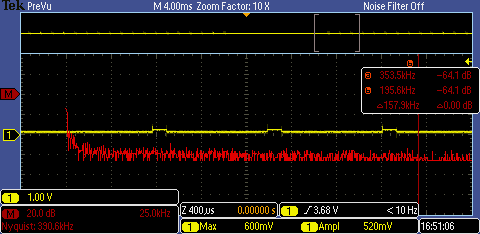
\includegraphics[width=\pic]{scope/ir_fft}
\caption{Frequency spectrum of noise}
\label{noise}
\end{figure}


\paragraph{(d) Motor} DC Motor measurements in Table-\ref{tab3}
\begin{table}
\center
  \begin{tabular}{|c|c|c|}
    \hline
    \multicolumn{3}{|c|}{DC Motor measurements} \\
    \hline
    Condition & Voltage across motor & Current \\
    \hline
	no-load				&	4.41v &	32mA \\
	with rubber wheel	&	4.42v &	34mA \\
	wheel \& on carpet	&   4.42v & 100mA \\
    \hline
  \end{tabular}
  \caption{DC motor measurements}
  \label{tab3}
\end{table}


\paragraph{(e) CAN scope picture} Below is a CAN packet measured at the CANH bus (yellow) and the microcontroller output (blue). It can be observed that the CANH signal is a inverted version of the microcontroller output, however the 
microcontroller output is changing between 0 and $3.3 \, V$, and the CANH signal is changing between about 2.5 and $3.8 \, V$.
Also, the length of a typical packet is $ 161.7 \, \mu s $

\setlength{\pic}{0.8\textwidth}
\begin{figure}[htp]
\center
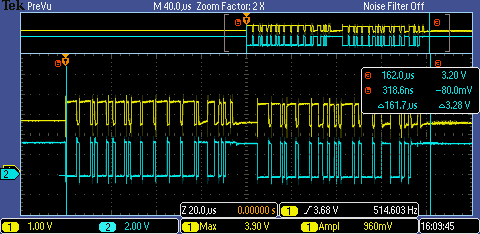
\includegraphics[width=\pic]{scope/CAN_packet}
\caption{Scope trace of a typical CAN packet}
\label{trace}
\end{figure}


\paragraph{(f) CAN Network bandwidth} We set the CAN network bit rate at $ 1 Mbit $ and decrease the sampling period of
IR sensor. The result is shown in Table-\ref{tab4}.

\begin{table}
\center
  \begin{tabular}{|c|c|}
    \hline
    \multicolumn{2}{|c|}{CAN Bandwidth} \\
    \hline
    Sampling Rate  & Data Lost \\
    \hline
	100 ms &   No \\
	10 ms  &   No \\
	5 ms   &   No \\
	4 ms   &   Yes \\
	3 ms   &   Yes \\
	2 ms   &   Yes \\
	1 ms   &   Yes \\
    \hline
  \end{tabular}
  \caption{Bandwith measurement}
  \label{tab4}
\end{table}

Therefore we deduct the maximum sampling rate the system can handle is $\frac{1}{5 \, ms} \times 4 \text{ bytes} = 800
 \text{ bytes/sec} $.
Considering the packet length measured in Figure-\ref{trace}, CAN network itself should not be the limiting factor.
The limiting factor is probably the execution speed of the data acquisition thread on the receiver side, which
needs to run a 51-point filter code for each IR sensor data.

\section{Analysis}

\paragraph{(1) What is one advantage of the Ping))) sensor over the GP2Y0A21YK sensor? \\ }

Ping))) outputs a PWM signal which duty cycles changes linearly with respect to the distance, so it's easier to convert the raw data to distance.

\paragraph{(2) What is one advantage of the \textbf{GP2Y0A21YK} sensor over the Ping))) sensor \\ }

\emph{GP2Y0A21YK} measures the distance by an analog voltage. It is easier to convert voltage to digital data using ADC compared to measure time in Ping.

\paragraph{(3) Describe the noise of the \textbf{GP2Y0A21YK} when measured with a spectrum analyzer. \\ }

The noise of the sensor is periodic square waves. An square wave contains all different frequencies, with Maximum amplitude at the frequency of the square wave.
You can see that the spectrum detects many different frequencies.

\paragraph{(4) Why did you choose the digital filters for your sensors? \\ }
What is the time constant for this filter? I.e., if there is a step change in input, how long until your output changes to at least 1/e of the final value?

Since the transition bandwidth of the analog filter is too large for a 2-pole low-pass filter, therefore we use the digital filter to filter out the noise. 

An analog filter with higher poles is more expensive. 

Since we're using a 51 point FIR filter, and $1/e = 0.36$, we need to sample about 17 points to get enough data to represent 0.36 of the input. 

Therefore, $\text{time constant } = \frac{17}{f_c} = 8.5 \, ms$

\paragraph{(5) Present an alternative design for your H-bridge and describe how your H-bridge is better or worse? \\ }

Alternate design is shown as Figure-\ref{hbridge}

Using our H-bridge is a trade-off. It is better in the simplicity of circuit design so to minimize risk of damaging circuit. Also it saves space. The alternate H-bridge is more sophisticated. This design gets a faster response time of the signal. However it's easier to cause problem and needs more components.

\setlength{\pic}{0.8\textwidth}
\begin{figure}[htp]
\noindent Alternative H-bridge circuit at Figure-\ref{hbridge}
\center
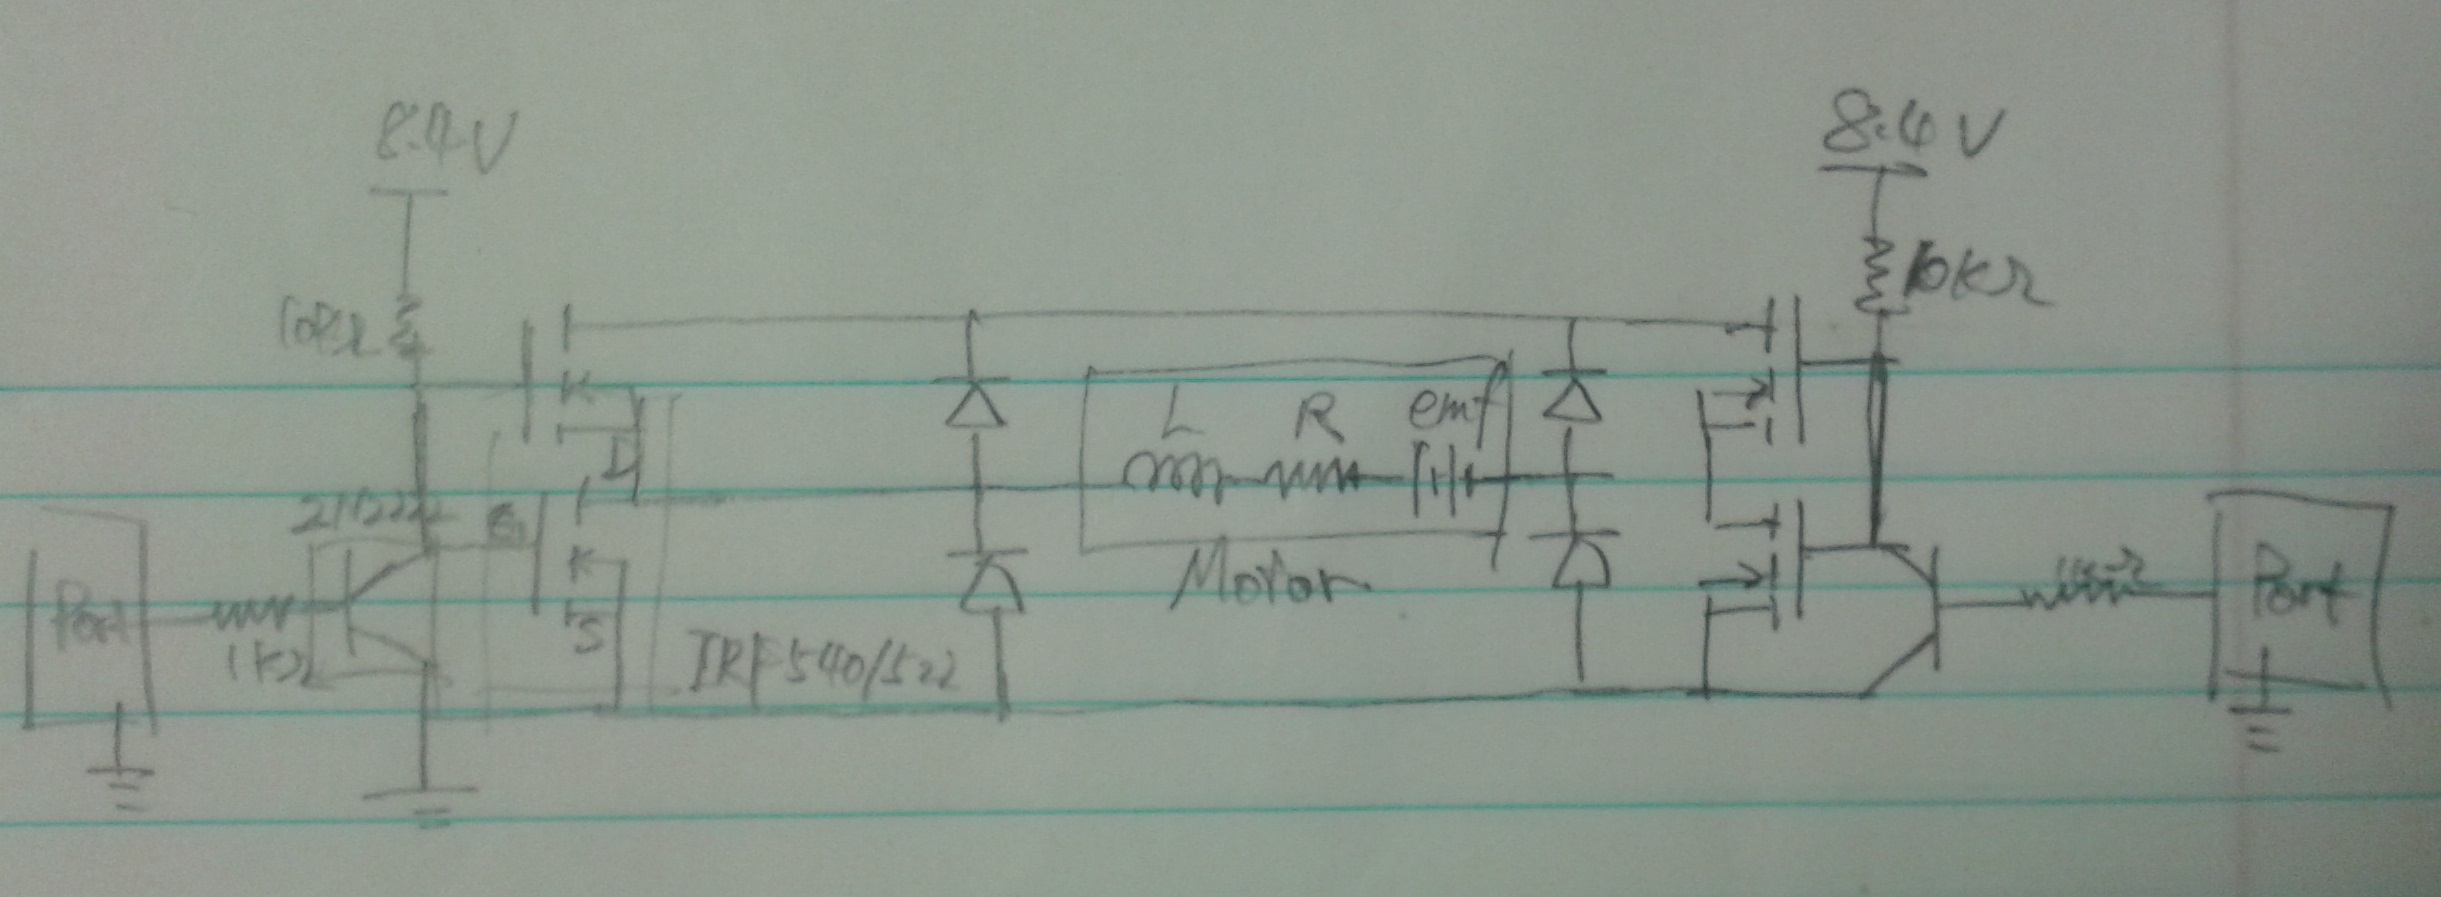
\includegraphics[width=\pic]{circuits/Alternate_H-bridge}
\caption{ }
\label{hbridge}
\end{figure}

\paragraph{(6) Give the single-most important factor in determining the maximum bandwidth on this distributed system.
Give the second-most important factor. Justify your answers.  \\ }

Since the system bandwidth was much less than the most possible theoretical bandwidth according to bit rate, the most important factor is the amount of time needed to prepare a package to be sent in the CAN driver, and the amount of time to receive and interpret an incoming package.

The second-most important factor is the bit-rate that determines the amount of time it takes for a single package to be transmitted over the bus.

\newpage
\section{Post-Mortem Team Evaluation}
Here we evaluate the Strengths and Weaknesses by teammate.

\subsection{Chen Cui}
\begin{itemize}
\item[Chen] not obvious in this lab; write code slowly
\item[YKH] Knowledge in C and embedded system; unknown
\item[MQ] perfectionist and experience in C; unknown
\item[Siavash] knowledge and experience; unknown
\item[ZY] knowledge in mechanical and hard-working; unknown
\end{itemize}

\subsection{Yen-Kai Huang}
\begin{itemize}
\item[Chen] Hardworking and experienced in motor interfacing; None
\item[YKH]  Experience in Embedded system and \LaTeX; Not very concentrated
\item[MQ]   Hardworking and easy to work with; Code style is not professional
\item[Siavash] Excellent embedded programmer; He is often busy with the senior design project
\item[ZY]   Very experienced in mechanical engineering and ability of hands-on work ; Lack of embedded experience
\end{itemize}

\subsection{Miao Qi}
\begin{itemize}
\item[Chen]	code is easy readable and in good style, good lab partner; None
\item[YKH]	His code is stylish and easy-readable, strong leadership; None
\item[MQ]	easy to communicate; code is not very portable
\item[Siavash]	Extremely strong coding skill, good organization skill; None
\item[ZY]	hard working, like to explore deeply; None
\end{itemize}

\subsection{Siavash Zangeneh Kamali}
\begin{itemize}
\item[Chen] Hardware interface, embedded systems; Not clear and concise in coding style
\item[YKH] Precise and clear coding style, good at programming, experienced in embedded systems ; Too much perfectionist
\item[MQ] on-time, hard working; Not clear and concise in coding style
\item[Siavash] good at programming, experienced in embedded systems ; Doesn't do things until the deadline is written
\item[ZY] Mechanical engineering stuff, hard working; Not clear and concise in coding style
\end{itemize}

\subsection{Yan Zhang}
\begin{itemize}
\item[Chen] 1. expert in the lab 2. working hard	;	(It's impossible for me to see you guys' weakness...)
\item[YKH]	1. expert in the lab 2. working hard	;	(It's impossible for me to see you guys' weakness...)
\item[MQ]	1. expert in the lab 2. working hard	;	(It's impossible for me to see you guys' weakness...)
\item[Siavash]	1. expert in the lab 2. working hard	;	(It's impossible for me to see you guys' weakness...)
\item[ZY]	1. never give up trying 2. working hard	;	1. little background in EE
\end{itemize}

\subsection*{Failure and Success in Communication}
We started out early with logistics and use new internet technology to improve our communication, for example
code repository and smartphone apps. The only thing preventing us from better communicating is the language barrier
because we all speak English as a second language, but despite this we are able to work beyond the nationality and
function well. Our success in communication is that we have been able to meet punctually and we have a strong
leadership and clear job assignment that makes everybody engaged and working.


\end{document}
